\documentclass[main.tex]{subfiles}
 
\begin{document}

\chapter{Scattering}
\PartialToc

limitazioni semiclassiche sul valore di l.
Da un punto di vista semiclassico la particella non pu\'o penetrare la bariera centrifuga
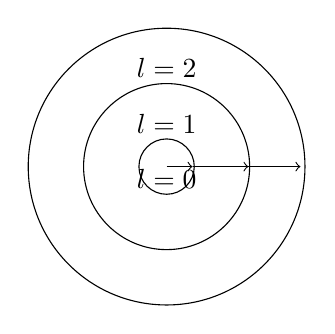
\begin{tikzpicture}
 \draw circle (10pt) node[label={[label distance=10pt]90:$l=0$},xshift=0,yshift=-25] (l0) {};
 \draw circle (30pt) node[label={[label distance=30pt]90:$l=1$},xshift=0,yshift=-25] (l1) {};
 \draw circle (50pt) node[label={[label distance=50pt]90:$l=2$},xshift=0,yshift=-25] (l2) {};
\draw[->] (0,0)--(0.33,0) node[label={[label distance=-2pt]100:$\lambdabar$},xshift=1,yshift=-5] {};
\draw[->] (0.33,0)--(1.04,0) node[label={[label distance=-2pt]100:$\lambdabar$},xshift=-1,yshift=-5] {};
\draw[->] (1.04,0)--(1.70,0) node[label={[label distance=-2pt]100:$\lambdabar$},xshift=-1,yshift=-5] {};
\end{tikzpicture}
If the particle with momentum p interact with impact parameter b the semiclassical relative angular momentum will be $l\hbar=pb$ cio\'e $b=l\frac{\hbar}{p}=l\lambdabar=\frac{1}{k}$; particles with semiclassical angular momentum $0\hbar\leq l\leq1 \hbar$  will interact with impact parameter $0\leq b\leq \lambdabar$ and thus over an area (cross section) at most $\pi\lambdabar^2$, with $1\hbar\leq l\leq2\hbar$ the cross section will be the ring of area $3\pi\lambdabar^2$. We can estimate the maximum impact parameter for nuclear scattering $R\approx R_1+R_2$ thus the maximum l is $\frac{R}{\lambdabar}$: $\sigma\approx\sum_{l=0}^{\frac{R}{\lambdabar}}(2l+1)\pi\lambdabar^2=\pi(R+\lambdabar)^2$.
La zona l-esima contiene particelle con parametro d'urto fra $l\lambdabar$ e $(l+1)\lambdabar$. Se $mvR\ll\hbar$ sono rilevanti solo le interazioni con l=0: $T=\frac{1}{2}mv^2\ll\frac{\hbar^2}{2mR^2}=\frac{\hbar^2c^2}{2mR^2c^2}\approx\frac{(200 MeV^2 fm^2)}{2*(1000 MeV) *(1 fm)^2}\approx 20 MeV$

\chapter{BB nucleosynthesis}
\PartialToc

\section{Proton capture on light elements}

\begin{itemize}
\item $D(^1H,\gamma)^3He$,$T_D\approx \SI{1e6}{\kelvin}$
\item $^7Li(^1H,^4He)^4He$, $T_{Li}\approx\SI{3e6}{\kelvin}$ 

\end{itemize}

\chapter{Nuclear burning in stars}
\PartialToc

\section{neutrino production}
\begin{itemize}
\item  Pair annihilation $\Pelectron+\APelectron\to\Pnue+\APnue$: $T>\SI{e9}{\kelvin}$ prob \num{e-19}
\item Photoneutrino: $\gamma+\Pelectron\to\Pelectron+\APnue+\Pnue$ in compton scattering
\item plasma neutrino: $\gamma_p\to\Pnue+\APnue$ - fotone accoppiato al moto collettivo degli elettroni in gas densi ionizzati - fotone \'e detto plasmone con massa efficace $\frac{h\omega_p}{2\pi c^2}$
\item Inelastic scattering of electrons in coulomb field produce photons but at vh densities and low T \Pnue\APnue pair - large atomic number
\item URCA: $(Z,A)+\Pelectron\to(Z-1,A)+\Pnue\to(Z,A)+\Pelectron+\APelectron$
\end{itemize}
\section{Fusion}
\begin{align*}
&\TDy{t}{X_i}=-A_im_HR_{ij}\\
&=-\rho\frac{X_iX_j}{m_HA_j}\frac{\exv{\sigma v}_{ij}}{1+\delta_{ij}}
\end{align*} 

\section{H burning: pp chain}

\section{H burning: CNO cycle}

\section{He burning}

\section{C-burning}

\section{photo-disintegration}
same as photo-diss but nuclear binding energy (from C-burning): 

\end{document}